\documentclass[11pt]{article}
\usepackage[textwidth=18.0cm, textheight=23.0cm, top=2.0cm]{geometry}
\usepackage{pst-all}
\usepackage{amssymb}
\usepackage{tikz}
\usepackage{underscore}\begin{document}
\pagestyle{empty}


ClassName: \underline{\textbf{Class_02.2bp-4}}
\par
BinSize: \underline{\textbf{30 × 30}}
\par
ReduceSize: \underline{\textbf{30 × 30}}
\par
TypeNum: \underline{\textbf{18}}
\par
Num: \underline{\textbf{20}}
\par
OutS: \underline{\textbf{900}}
\par
InS: \underline{\textbf{534}}
\par
Rate: \underline{\textbf{0.593}}
\par
UB: \underline{\textbf{1}}
\par
LB0: \underline{\textbf{1}}
\par
LB: \underline{\textbf{1}}
\par
LBWithCut: \underline{\textbf{1}}
\par
NodeCut: \underline{\textbf{0}}
\par
ExtendedNodeCnt: \underline{\textbf{1}}
\par
GenNodeCnt: \underline{\textbf{1}}
\par
PrimalNode: \underline{\textbf{0}}
\par
ColumnCount: \underline{\textbf{1}}
\par
TotalCutCount: \underline{\textbf{0}}
\par
RootCutCount: \underline{\textbf{0}}
\par
LPSolverCnt: \underline{\textbf{1}}
\par
PricingSolverCnt: \underline{\textbf{0}}
\par
BranchAndBoundNum: \underline{\textbf{1}}
\par
isOpt: \underline{\textbf{true}}
\par
TimeOnPrimal: \underline{\textbf{0.000 s}}
\par
TimeOnPricing: \underline{\textbf{0.000 s}}
\par
TimeOnRmp: \underline{\textbf{0.063 s}}
\par
TotalTime: \underline{\textbf{0.125 s}}
\par
\newpage


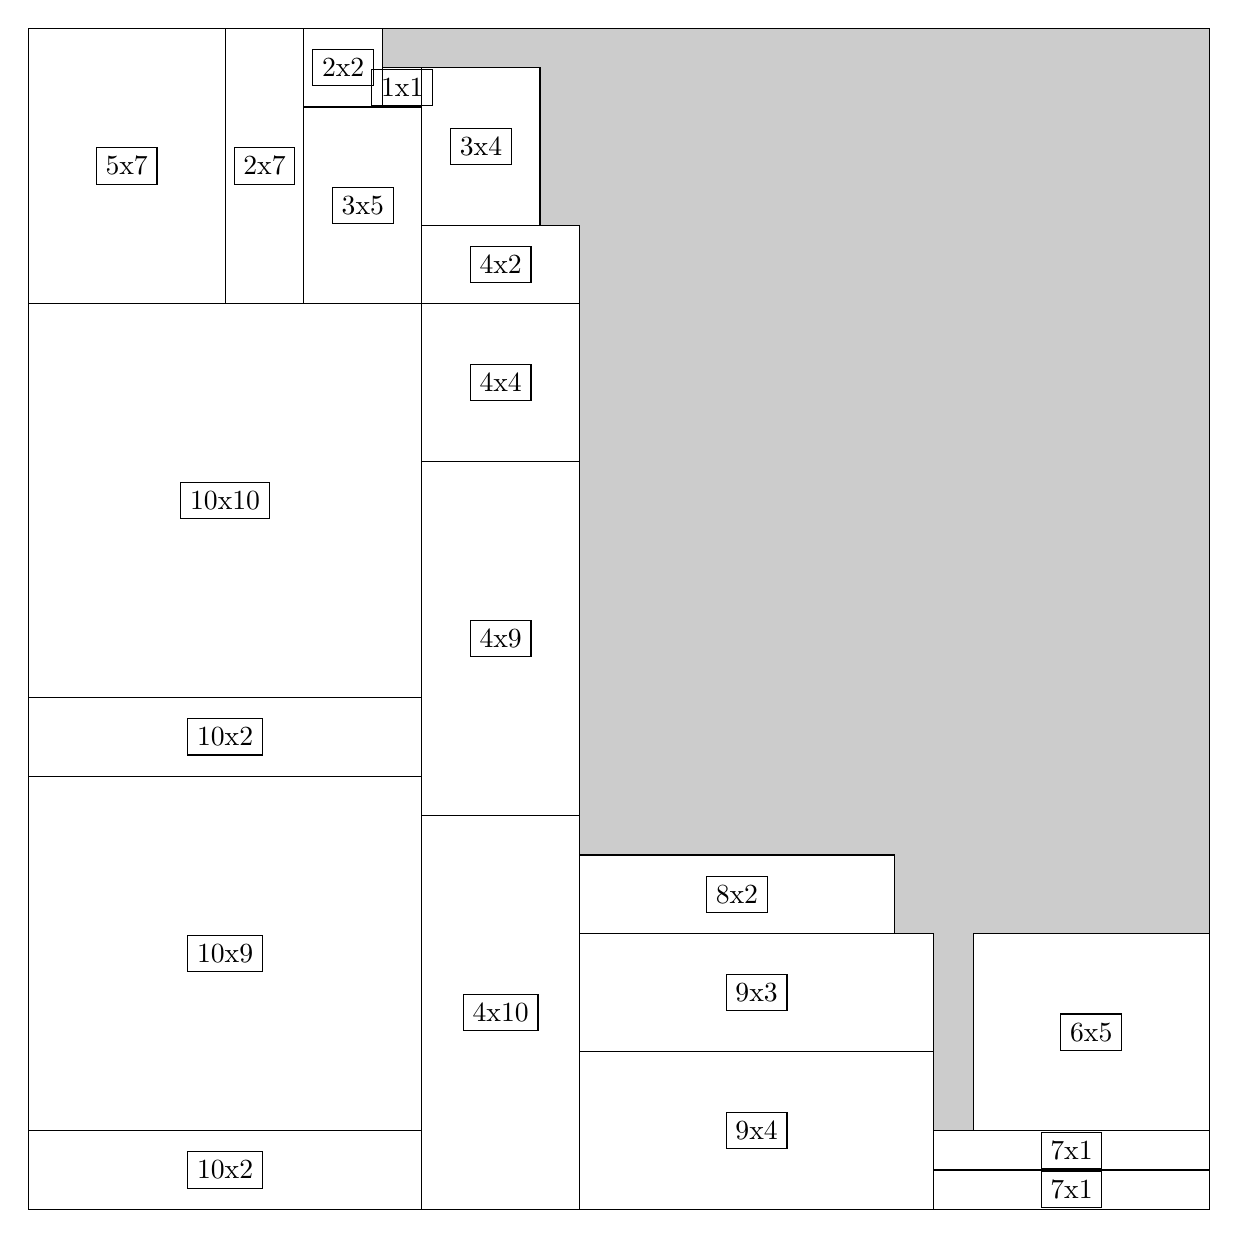
\begin{tikzpicture}[shorten >=1pt,scale=1.0,every node/.style={scale=1.0},->]
\tikzstyle{vertex}=[circle,fill=black!25,minimum size=14pt,inner sep=0pt]
\filldraw[fill=gray!40!white, draw=black] (0,0) rectangle (15.0,15.0);
\foreach \name/\x/\y/\w/\h in {10x2/0.0/0.0/5.0/1.0,10x9/0.0/1.0/5.0/4.5,4x10/5.0/0.0/2.0/5.0,9x4/7.0/0.0/4.5/2.0,4x9/5.0/5.0/2.0/4.5,5x7/0.0/11.5/2.5/3.5,6x5/12.0/1.0/3.0/2.5,9x3/7.0/2.0/4.5/1.5,10x2/0.0/5.5/5.0/1.0,10x10/0.0/6.5/5.0/5.0,8x2/7.0/3.5/4.0/1.0,4x4/5.0/9.5/2.0/2.0,3x5/3.5/11.5/1.5/2.5,2x7/2.5/11.5/1.0/3.5,3x4/5.0/12.5/1.5/2.0,4x2/5.0/11.5/2.0/1.0,7x1/11.5/0.0/3.5/0.5,7x1/11.5/0.5/3.5/0.5,2x2/3.5/14.0/1.0/1.0,1x1/4.5/14.0/0.5/0.5}
\filldraw[fill=white!40!white, draw=black] (\x,\y) rectangle node[draw] (\name) {\name} ++(\w,\h);
\end{tikzpicture}


w =10 , h =2 , x =0 , y =0 , v =20
\par
w =10 , h =9 , x =0 , y =2 , v =90
\par
w =4 , h =10 , x =10 , y =0 , v =40
\par
w =9 , h =4 , x =14 , y =0 , v =36
\par
w =4 , h =9 , x =10 , y =10 , v =36
\par
w =5 , h =7 , x =0 , y =23 , v =35
\par
w =6 , h =5 , x =24 , y =2 , v =30
\par
w =9 , h =3 , x =14 , y =4 , v =27
\par
w =10 , h =2 , x =0 , y =11 , v =20
\par
w =10 , h =10 , x =0 , y =13 , v =100
\par
w =8 , h =2 , x =14 , y =7 , v =16
\par
w =4 , h =4 , x =10 , y =19 , v =16
\par
w =3 , h =5 , x =7 , y =23 , v =15
\par
w =2 , h =7 , x =5 , y =23 , v =14
\par
w =3 , h =4 , x =10 , y =25 , v =12
\par
w =4 , h =2 , x =10 , y =23 , v =8
\par
w =7 , h =1 , x =23 , y =0 , v =7
\par
w =7 , h =1 , x =23 , y =1 , v =7
\par
w =2 , h =2 , x =7 , y =28 , v =4
\par
w =1 , h =1 , x =9 , y =28 , v =1
\par
\newpage


\end{document}